\begin{figure}[htbp]
\section*{ ZFX}
\centering
\begin{subfigure}[b]{0.95\textwidth}
\centering
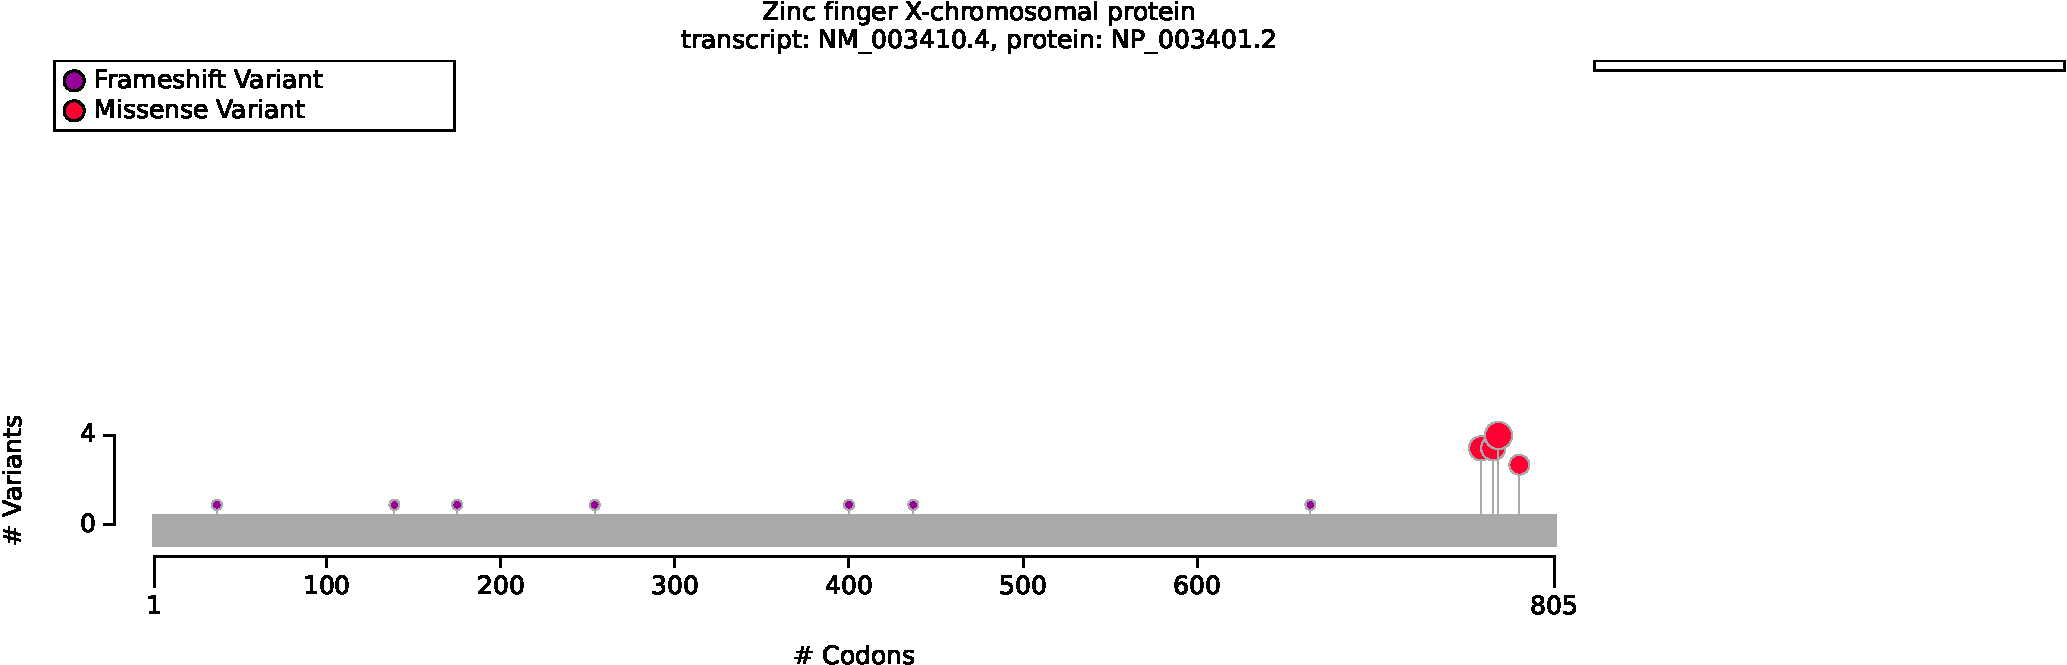
\includegraphics[width=\textwidth]{ img/ZFX_protein_diagram.pdf} 
\captionsetup{justification=raggedright,singlelinecheck=false}
\caption{Distribution of variants in ZFX}
\end{subfigure}

\vspace{2em}
\begin{subfigure}[b]{0.95\textwidth}
\centering
\resizebox{\textwidth}{!}{
\begin{tabular}{llllrr}
\toprule
HPO term & missense & other & p-value & adj. p-value\\
\midrule
Hyperparathyroidism [HP:0000843] & 7/9 (78\%) & 0/5 (0\%) & 0.021 & 0.021\\
\bottomrule
\end{tabular}
}
\captionsetup{justification=raggedright,singlelinecheck=false}
\caption{ 
Fisher Exact Test performed to compare HPO annotation frequency with respect to missense and other. Total of
1 test was performed. }
\end{subfigure}
\vspace{2em}
\begin{subfigure}[b]{0.95\textwidth}
\centering
\resizebox{\textwidth}{!}{
\begin{tabular}{llllrr}
\toprule
Genotype (A) & Genotype (B) & total tests performed & significant results\\
\midrule
missense & other & 225 & 0\\
\bottomrule
\end{tabular}
}
\captionsetup{justification=raggedright,singlelinecheck=false}
\caption{Fisher Exact Test performed to compare HPO annotation frequency with respect to genotypes.}
\end{subfigure}

\vspace{2em}
\caption{ The cohort comprised 19 individuals (4 females, 14 males, 1 with unknown sex). A total of 203 HPO terms were used to annotate the cohort. Disease diagnosis: Intellectual developmental disorder, X-linked syndromic 37 (OMIM:301118). The small cohort size and the fact that the majority of the ZFX variants were private to each proband or 
family made the assessment of genotype-phenotype correlation difficult. A recent report of a
germline ZFX missense variant in a patient With primary hyperparathyroidism suggested the hypothesis of
testing for correlation between missense variants and hyperparathyroidism \cite{PMID_38325380,PMID_39056049}. A total of 11 unique variant alleles were found in \textit{ZFX} (transcript: \texttt{NM\_003410.4}, protein id: \texttt{NP\_003401.2}).}
\end{figure}
